% !TEX root = ../../I4PRJ, Grp3 - Rapport.tex
\subsubsection{Implementering}
Den visuelle Implementering af websitet med ASP.NET MVC, den visuelle implementering er skrevet i HTML og CSS. Clientside funktionaliteten er skrevet i JavaScript slutteligt er der brugt razor, som er et server-side markup sprog.

\begin{figure}
	\centering
	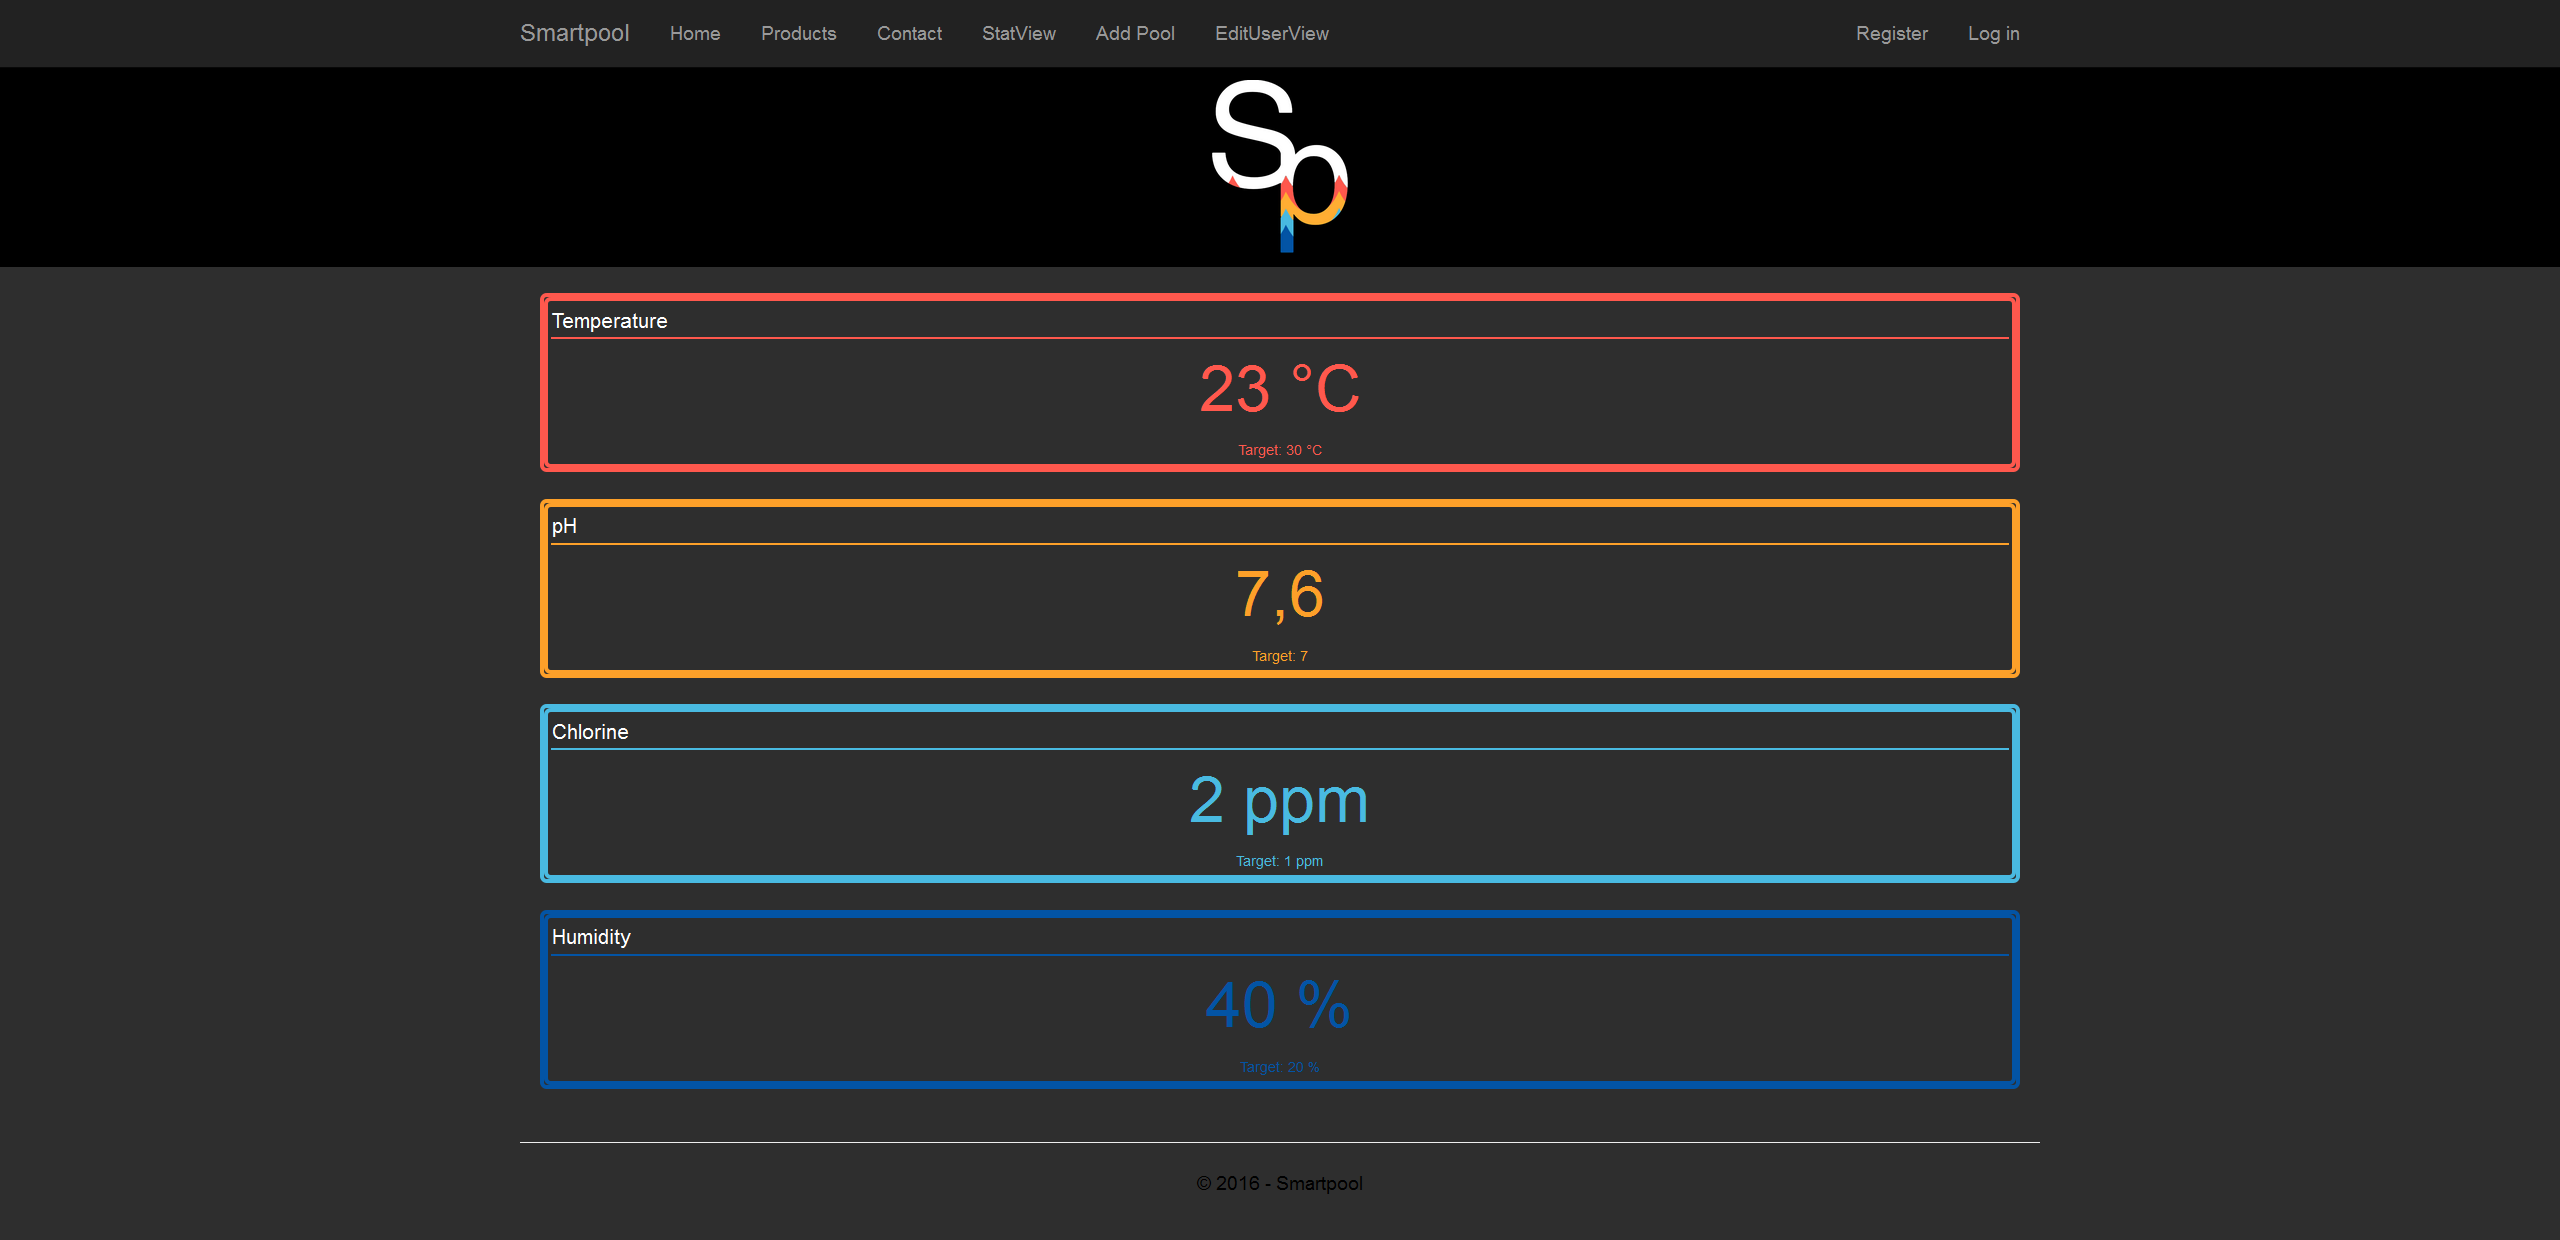
\includegraphics[width=1.0\linewidth]{figs/implementering/web_statview}
	\caption{Web StatView}
	\label{fig:webstatview}
\end{figure}

\paragraph{LoginView}
LoginView ses på figuren nedenfor:

\begin{figure}
	\centering
	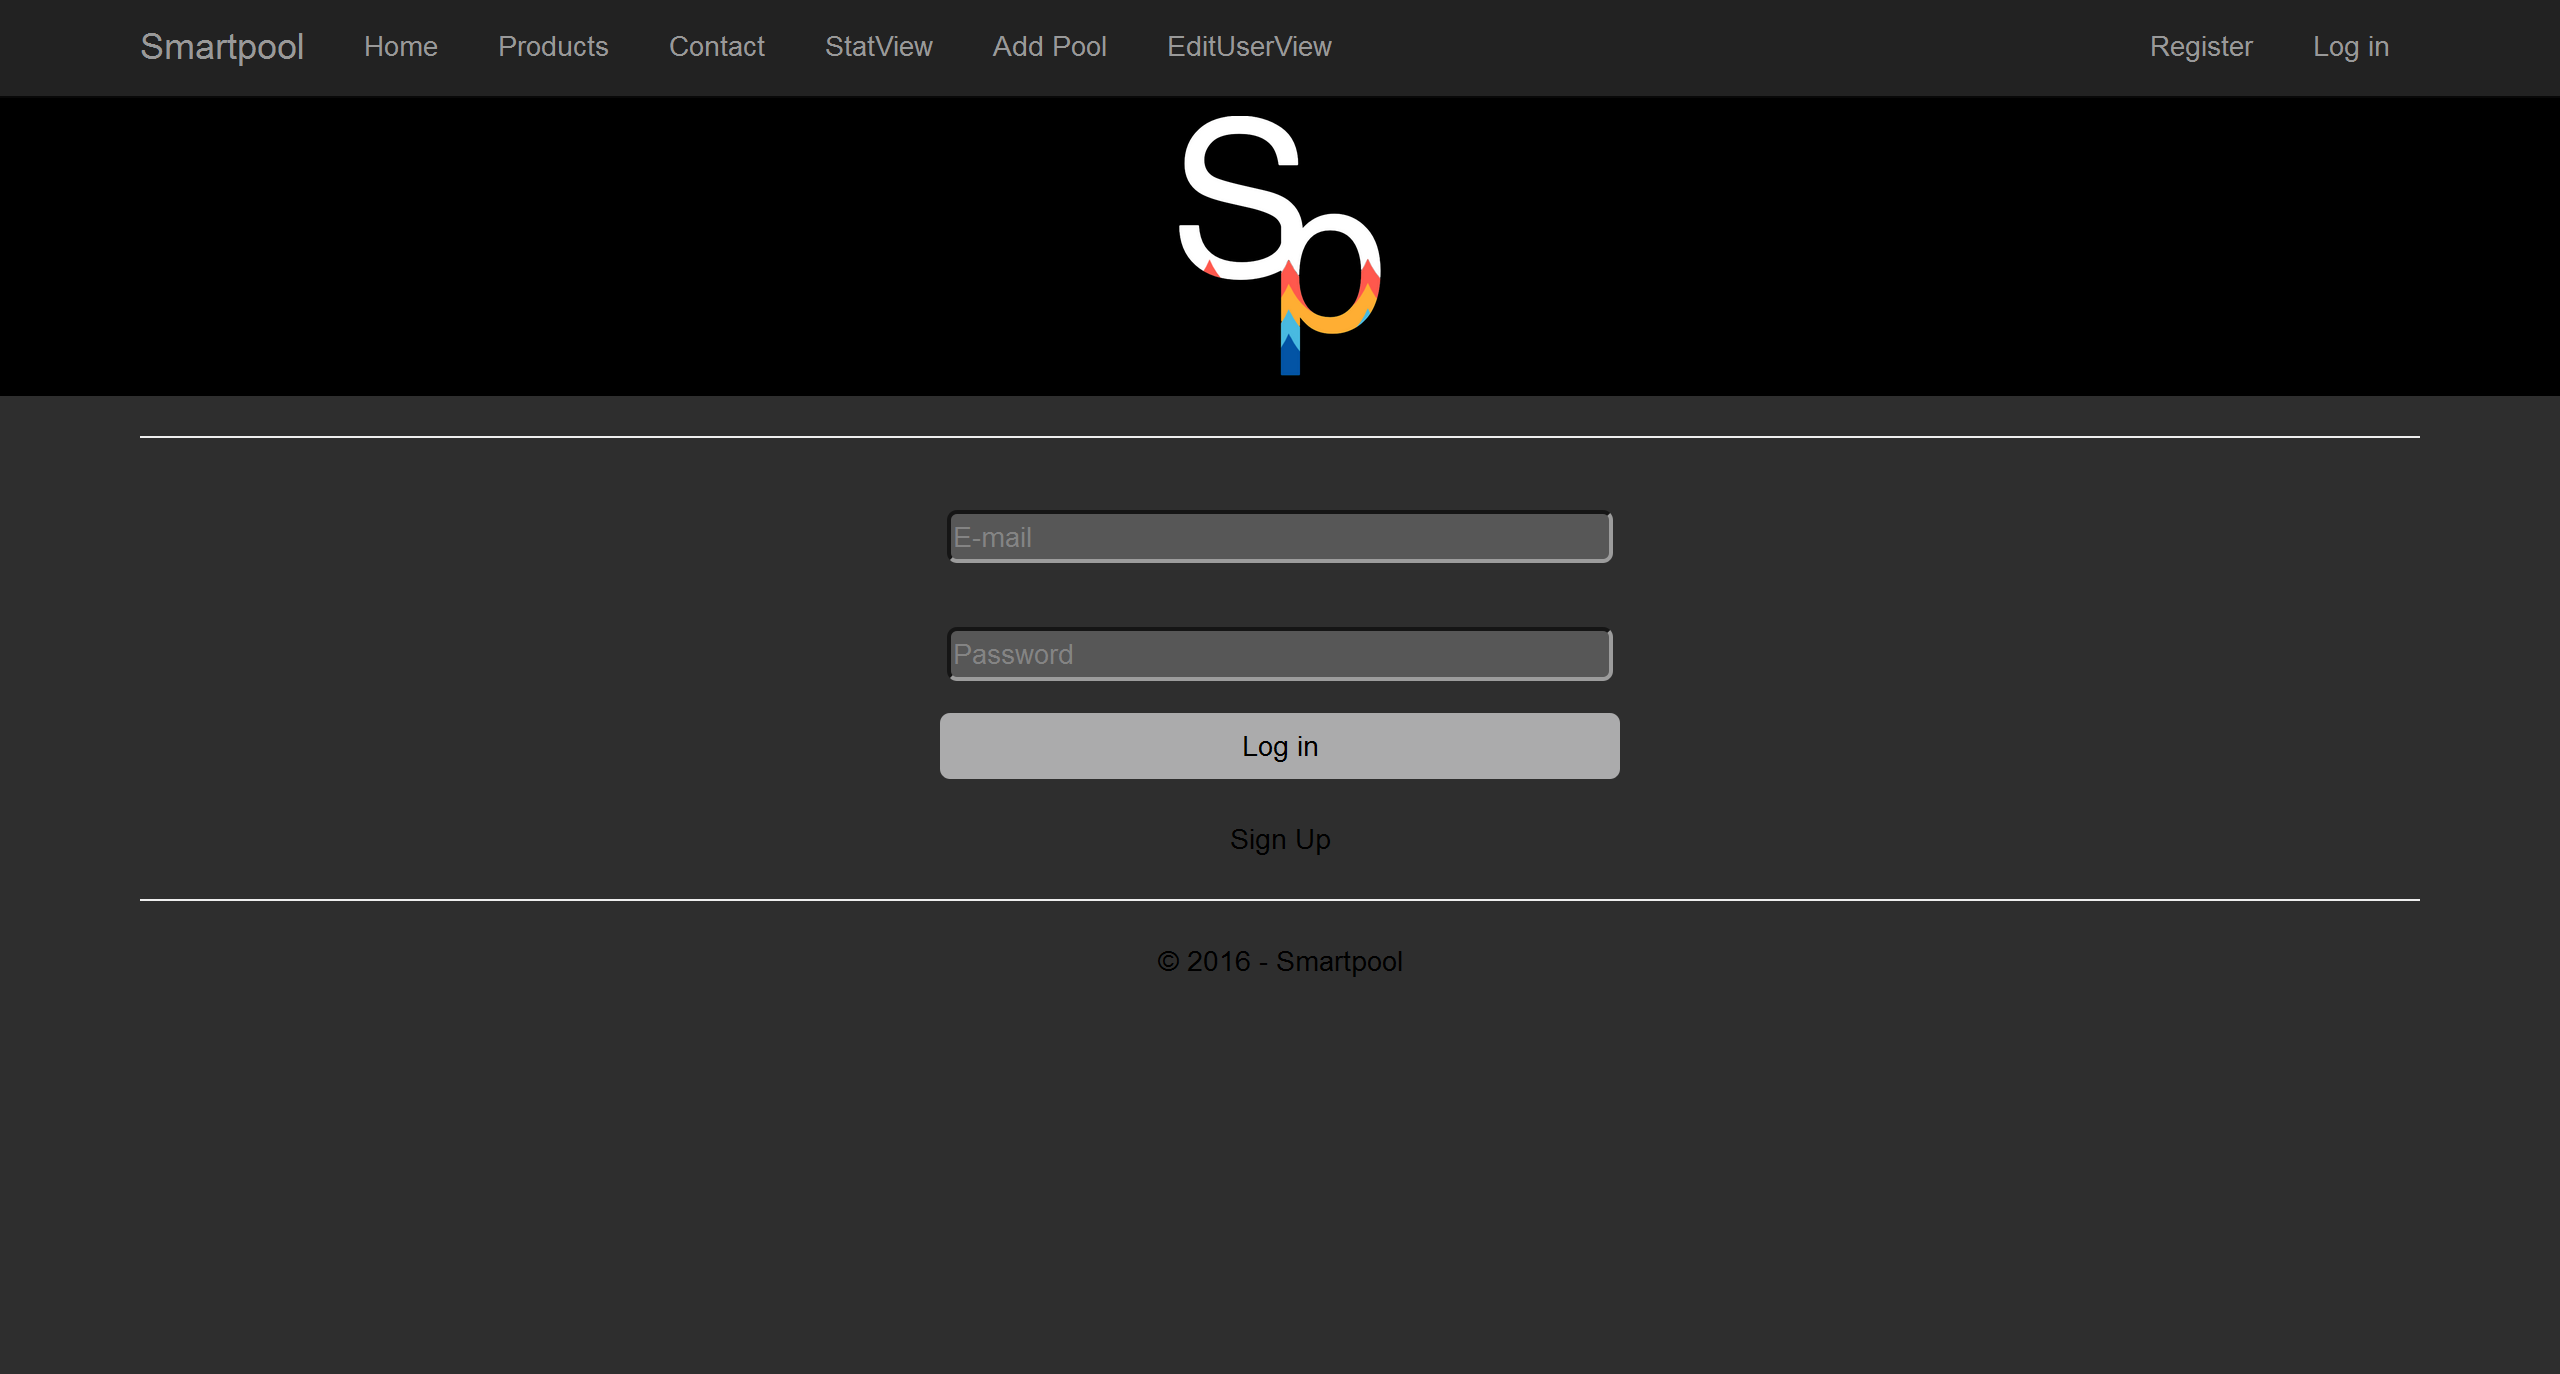
\includegraphics[width=1.0\linewidth]{figs/implementering/web_login}
	\caption{Web LoginView}
	\label{fig:webloginview}
\end{figure}

Når login knappen kaldes AccountController som håndtere login request. Email og password sendes til presenter. Når svaret på login returneres, kaldes LoginAccepted som implementeres i AccountController. LoginAccepted redirects til et andet url på web serveren. For mere om implementering og kodeeksempel se dokumentationen.

\paragraph{AddPoolView}
AddPoolView ses på figuren nedenfor:

\begin{figure}
	\centering
	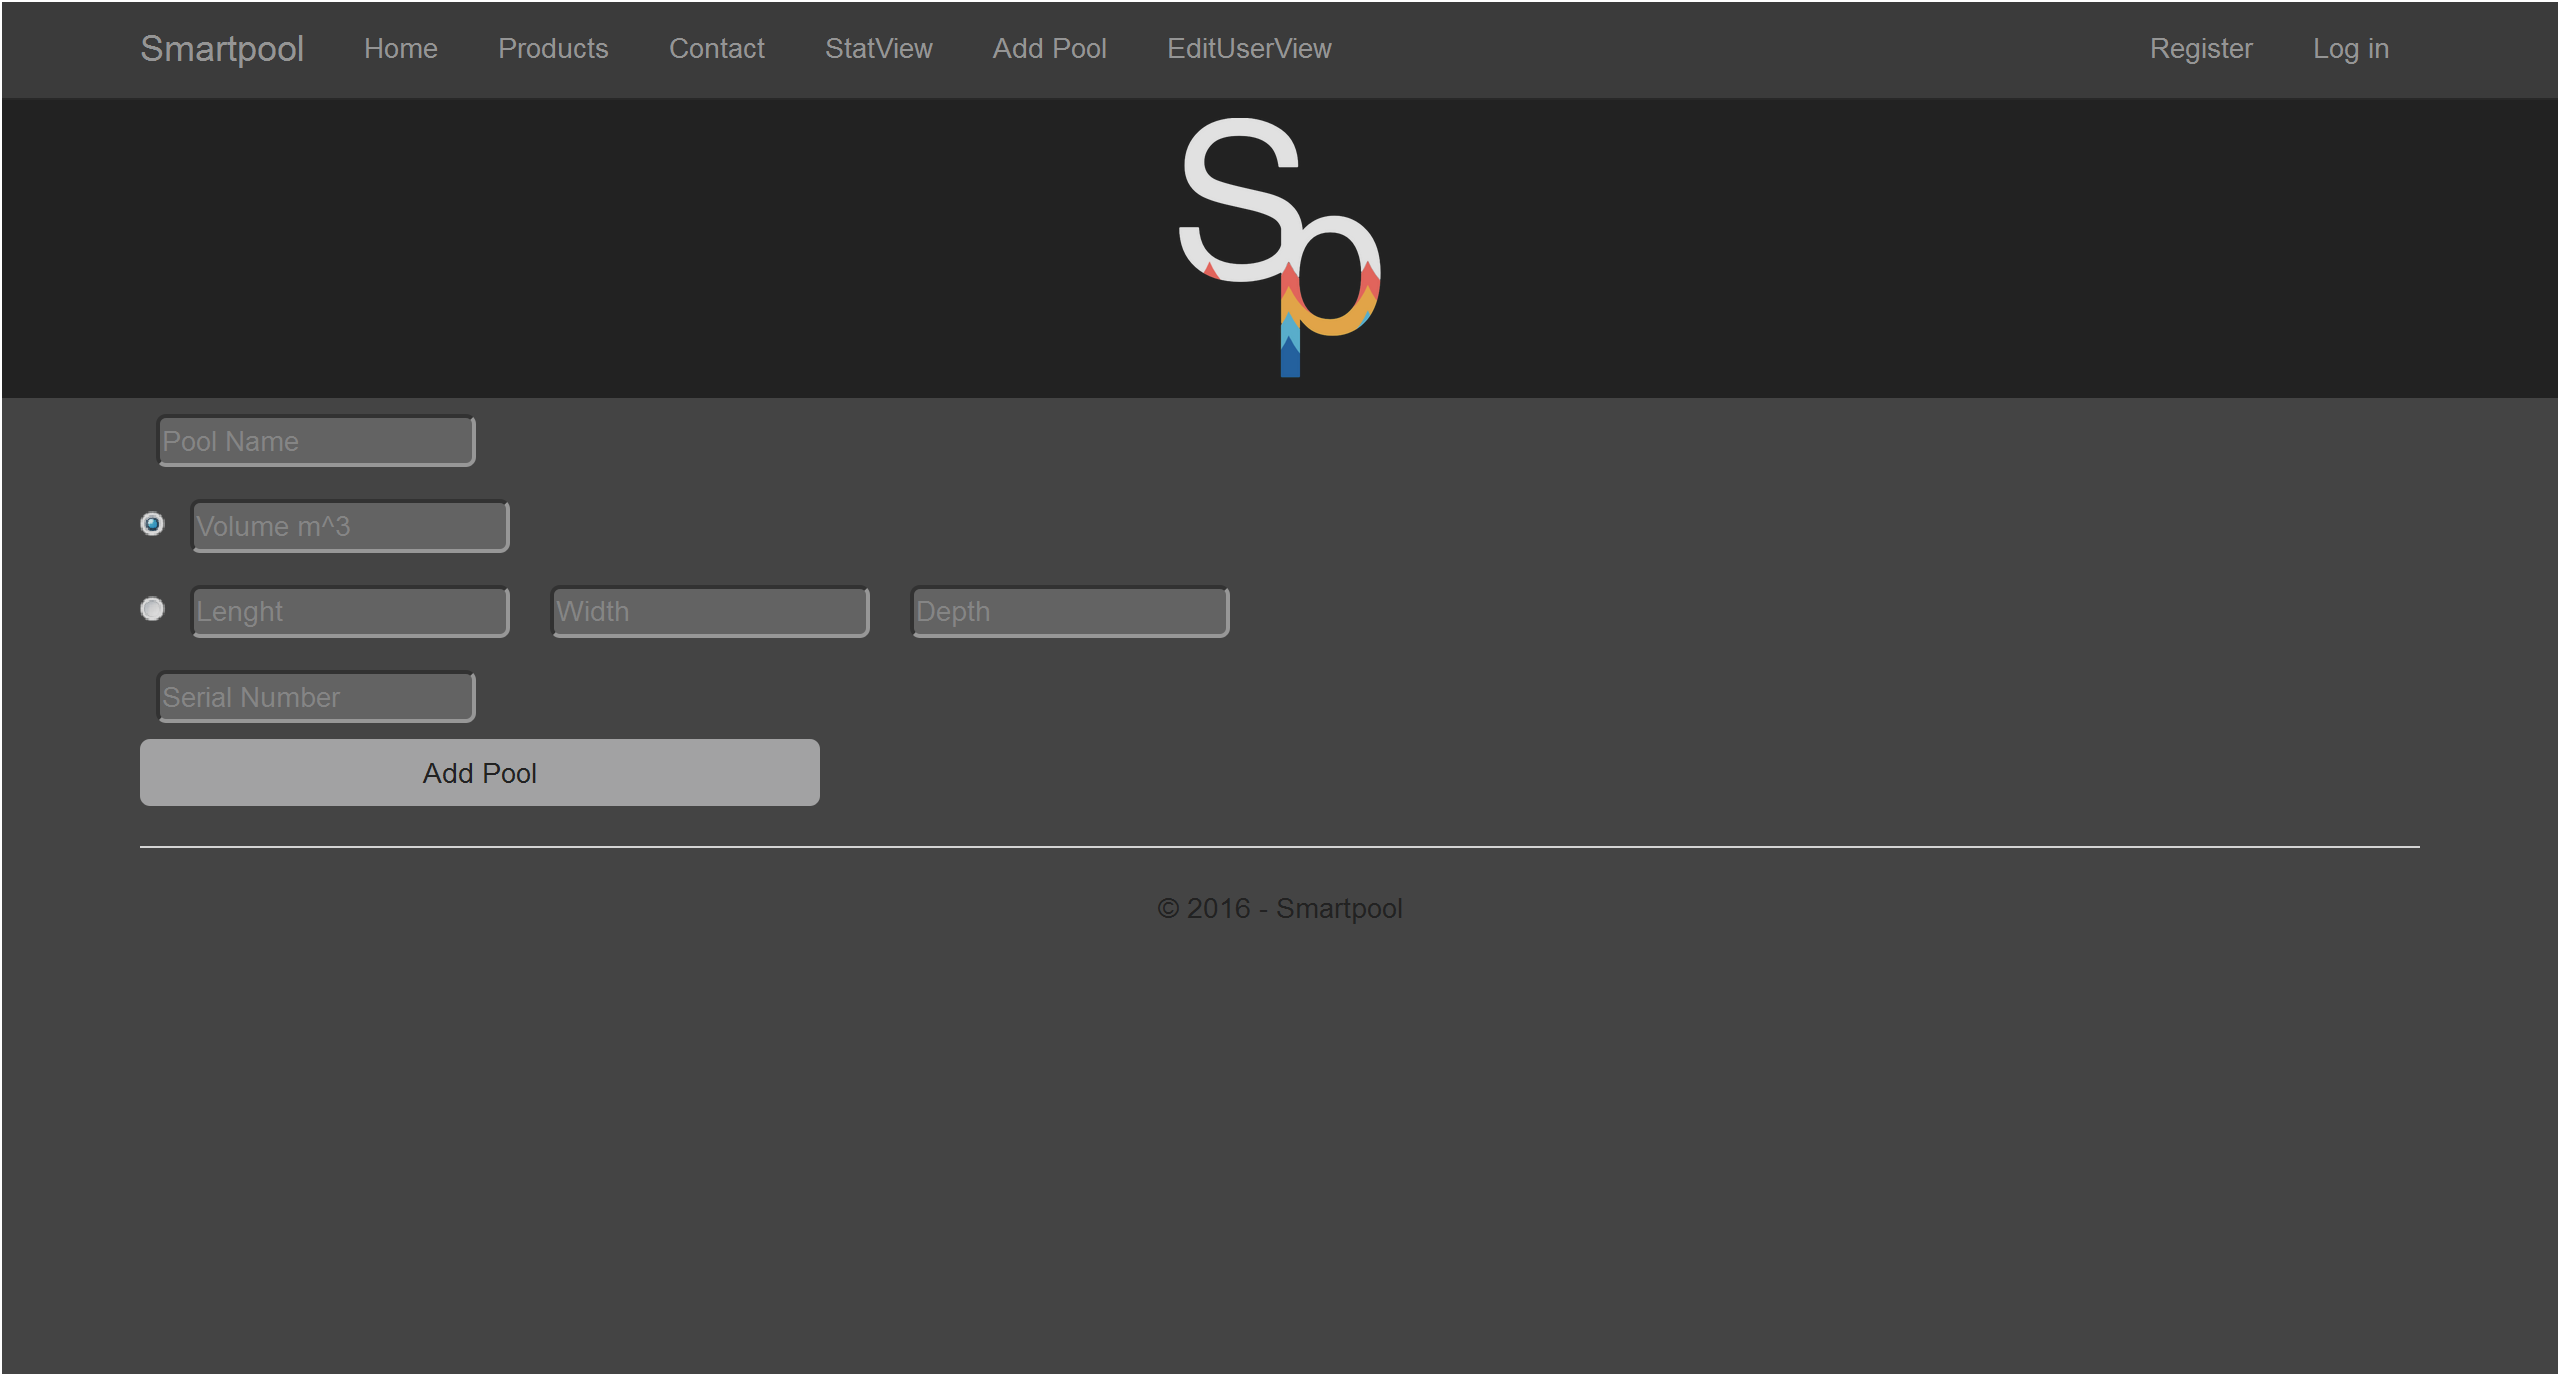
\includegraphics[width=1.0\linewidth]{figs/implementering/web_addpoolview}
	\caption{Web AddPoolView}
	\label{fig:webaddpoolview}
\end{figure}

Brugeren kan vælge enten at indtaste volumen eller dimensioner, ved at vælge på radioknapperne. Når den ene er valgt skal den anden mulighed ikke være tilgængeligt. Der håndterer scriptet enableTxtBox. 

Er brugeren begyndt at indtaste volumen, men ombestemmer sig, så skal tekstfeltet tømmes, det håndteres af scriptet clearText. 

Der er ikke muligt for brugeren at indtaste andet end tal, det håndterer scriptet isNumber. Disse JavaScripts implementeres i viewet. Mere om implementering og eksempler se dokumentation.

For implementering af andre views henvises til projektdokumentationen. 